\chapter{Обзор средств разработки и проектирование приложения}
\label{cha:design}

\section{Использованное оборудование}
В таблице \ref{tab:tab1} приведены краткие технические характеристики оборудования, на котором производилась разработка приложения.

\begin{table}
	\centering
	\begin{tabular}{ |l|l|c|c| } 
		\hline
		Процессор & Intel(R) Core(TM) i5-4200H \\
		\hline
		Базовая тактовая частота процессора & 2.8 GHz \\
		\hline
		Количество ядер процессора & 2 \\
		\hline
		Объем ОЗУ & 8 Гб \\
		\hline
		Операционная система & Windows 10 Pro \\ 
		\hline
	\end{tabular}
	\caption{Технические характеристики оборудования}
	\label{tab:tab1}
\end{table}

\section{Инструменты разработки}

В качестве среды разработки был выбран текстовый редактор Visual Studio Code. Данный выбор обусловлен в первую очередь легковесностью по сравнению с полноценными интегрированными средами разработки (WebStorm, Visual Studio и~др.) и богатым разнообразием дополнительных расширений. Кроме того, данный редактор является кросплатформенным и распространяется бесплатно, а также имеет интеграцию с системой контроля версий Git.

\subsection{Клиентская часть приложения}

Появление JavaScript в 1995 году сделало возможным применение современных веб-приложений~--- приложений, с которыми можно взаимодействовать без перезагрузки страницы при каждом действии пользователя. Изначально он создавался для придания интерактивности веб-страницам, но, как показывает картина, на сегодняшний день JavaScript является самым распространенным решением для разработки приложений на стороне клиента и одним из самых популярных~--- на серверной стороне.

Примечательно то, что JavaScript~--- это не только язык, но и целая инфраструктура, состоящая из огромного количества фреймворков и библиотек. Их разнообразие столь колоссально, что выделить лучший становится невозможно, поэтому выбор фреймворка для того или иного решения остается личным предпочтением разработчика или компании. А вручную описывать манипуляции с иерархической структурой гипертекстовой разметки на <<ванильном>> JavaScript является довольно ресурсоемкой задачей даже для небольшого проекта. Хотя бы по этой причине в современном мире есть огромная необходимость во фреймворках.

Опираясь на выводы, сделанные в разделе 1, было принято решение о реализации клиентской части в виде одностраничного приложения с использованием фреймворка. На момент написания данной работы наиболее популярными фреймворками для создания одностраничных приложений являются Angular, React и Vue.js.

В данном проекте для обеспечения работы клиентской части приложения был выбран фреймворк \textbf{Vue.js} \cite{vuejs}. Данный выбор обусловлен наличием у автора этой работы опыта разработки на выбранном фреймворке. Стоит выделить основные преимущества, которыми он обладает:

\begin{itemize}
	\item \textbf{Реактивность.} Состояние интерфейса приложения автоматически реагирует на изменение данных;
	\item \textbf{Легковесность.} Минимизированный и сжатый файл Vue.js занимает примерно 24 Кб, что довольно скромно для прогрессивного фреймворка;
	\item \textbf{Производительность.} Vue.js использует Virtual DOM: все операции выполняются с не привязанным к браузеру представлением DOM, после чего внесенные изменения копируются на саму страницу, что и обеспечивает высокую производительность \cite{stefankrause};
	\item \textbf{Интеграция.} Vue.js легко адаптировать и внедрить в уже существующий проект, не оказывая при этом негативного влияния на всю систему;
	\item \textbf{Масштабируемость.} Vue.js позволяет создавать крупные шаблоны и переиспользовать их, что значительно сокращает затраты на разработку;
	\item \textbf{Низкий порог вхождения.} Любое приложение на Vue.js пишется с помощью знакомых любому веб-разработчику технологий: HTML для разметки страницы, CSS для стилизации элементов и JavaScript для обеспечения интерактивного взаимодействия с конечным пользователем.
\end{itemize}

Также на клиентской части приложения используется официальный роутер Vue Router \cite{vuerouter}, отвечающий за маршрутизацию одностраничного приложения, и библиотека управления состоянием Vuex \cite{vuex}. В качестве вспомогательных библиотек разрабатываемого приложения выступают такие библиотеки, как Axios \cite{axios}, Vuelidate \cite{vuelidate} и Vue Material \cite{vuematerial}.

\subsection{Серверная часть приложения}

При создании веб-приложения основную роль занимает разработка серверной части. Есть два варианта: развернуть сервер самостоятельно или использовать уже готовое решение. Для поставленных целей вполне подойдет \textbf{Firebase}~--- продукт компании Google для быстрого создания мобильных и веб-приложений \cite{firebase}.

Firebase включает в себя множество полезных сервисов, но основным является облачная система управления базами данных класса NoSQL, позволяющая хранить и синхронизировать данные между несколькими пользователями. Firebase еще хорош тем, что автоматически масштабируется и после внедрения в проект позволяет сразу же приступать к разработке. Для полноты картины ниже будут перечислены все сервисы Firebase, использованные в данной работе:

\begin{itemize}
	\item \textbf{Firebase Auth.} Данный сервис позволяет аутентифицировать пользователей. Также доступна система управления пользователями, в соответствии с которой можно включить аутентификацию с помощью электронной почты и пароля;
	\item \textbf{Cloud Firestore.} Гибкая, масштабируемая облачная база данных, которая позволяет хранить данные и легко получать к ним доступ, а также следить за изменениями в режиме реального времени;
	\item \textbf{Firebase Storage.} Хранилище обеспечивает доступ к файлам пользователей. Можно использовать этот сервис для хранения пользовательского контента, например, различных медиафайлов;
	\item \textbf{Firebase Hosting.} Этот сервис поддерживает размещение статических файлов (HTML, CSS, JavaScript и т.~д.) и позволяет произвести быструю развертку приложения одной командой.
\end{itemize}

\section{Концепт приложения}

Исходя из проведенного анализа в разделе 1 следует определить основной процесс, благодаря которому пользователь сможет усваивать знания и взаимодействовать с приложением в целом. Этот процесс в разрабатываемом приложении выглядит следующим образом:

\begin{itemize}
	\item чтобы имплементировать метод параллельного чтения, в разрабатываемом приложении необходим модуль, отвечающий за книги и их части: посредством чтения книг с параллельным переводом пользователь сможет добавлять не знакомые ему слова в свой личный словарь для изучения;
	\item для имплементации метода интервальных повторений в разрабатываемом приложении необходим модуль, отвечающий за пользовательские данные: непосредственно при чтении книг все добавленные слова будут помещены именно в этот модуль, в котором также будет определена логика запоминания слов;
	\item чтобы пользователи могли делиться опытом изучения иностранного языка и задавать вопросы друг другу, в разрабатываемом приложении необходимы модули, отвечающие за статьи и форум, которые помогут повысить мотивацию к обучению.
\end{itemize}

\section{Задачи и требования}

С учетом выбранных инструментов разработки и общей идеи приложения, обозначенных в двух предыдущих подразделах, следует определить основной функционал, которым должно обладать разработанное приложение.

Веб-приложение должно обеспечивать аутентификацию пользователей: получение введенных из формы данных и сохранение входа после перезагрузки страницы, а также обработка ошибок и защита от несанкционированного входа.

Также в разрабатываемом приложении должен быть компонент, отвечающий за функциональность личного кабинета:

\begin{enumerate}
	\item возможность изменять личные данные пользователя: имя, электронную почту, пароль и изображение профиля;
	\item просмотр персональной информации, связанной с обучением: набор слов для изучения, представленный в виде таблицы, а также все книги, добавленные пользователем.
\end{enumerate}

Помимо этого в веб-приложении должна быть разработана система форумов, состоящая из разделов, каждый из которых нацелен на определенную тематику: 

\begin{enumerate}
	\item возможность фильтрации тредов по трем типам: треды пользователя, решенные и нерешенные треды;
	\item возможность создавать, редактировать и удалять треды, а также оставлять комментарии к ним (комментарии также можно удалять);
	\item автор треда может помечать один из комментариев к треду как решение своей проблемы.
\end{enumerate}

Плюс ко всему разрабатываемое приложение должно иметь компонент, отвечающий за систему пользовательских статей:

\begin{enumerate}
	\item возможность фильтрации статей по трем типам: статьи пользователя, статьи людей, на которых пользователь подписан, и понравивишеся статьи;
	\item возможность создавать, редактировать и удалять статьи, а также оставлять комментарии к ним (комментарии также можно удалять).
\end{enumerate}

Вдобавок в приложении необходим компонент, отвечающий за просмотр списка книг и возможность поиска и фильтрации по уровню подготовки, а также компонент для просмотра подробной информации о каждой отдельно взятой книге и ее частях с возможностью ее добавления в личную библиотеку.

Чтение частей книги должно осуществляться с возможностью переводить отдельные слова или целые предложения и добавлять их в личный словарь для изучения.

Также в веб-приложении необходим динамический тренажер для запоминания добавленных пользователем слов с возможностью озвучивания слова.

Кроме всего прочего для разрабатываемого приложения необходимо обеспечить безопасность данных посредством настройки правил для базы данных и защиты маршрутов.

И, наконец, разрабатываемое приложение должно быть снабжено адаптивным пользовательским интерфейсом.


\section{Архитектура приложения}

С учетом выбранных и обоснованных инструментов разработки, обозначенных в данном разделе, была также определена архитектура клиентской и серверной частей веб-приложения. Она изображена на рис.~\ref{fig:arch} и представляет из себя прямое взаимодействие веб-приложения на Vue.js с сервисами Firebase через его API. В разделе 3 описано, как именно и с помощью каких инструментов осуществляется данное взаимодействие.

\clearpage

\begin{figure}[h]
	\centering
	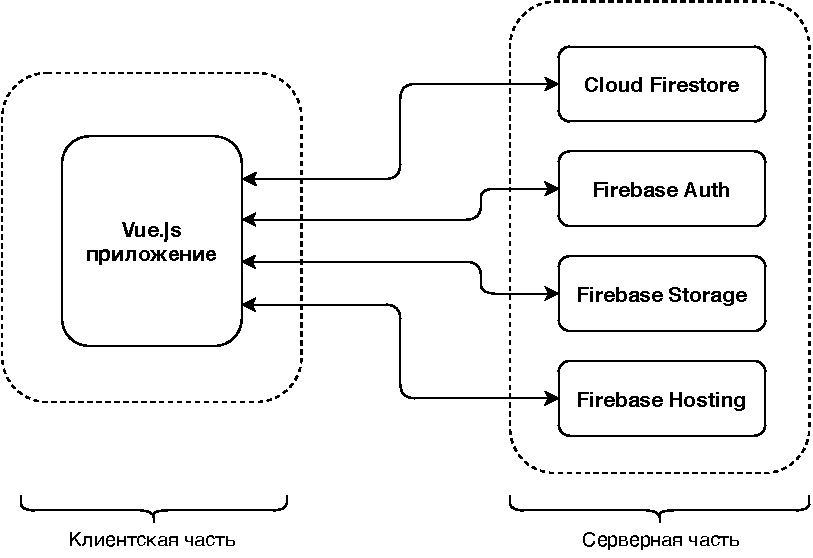
\includegraphics[width=\textwidth, keepaspectratio]{figures/arch}
	\caption{Архитектура приложения}
	\label{fig:arch}
\end{figure}

\section{Вывод}

Таким образом, опираясь на выводы из предыдущего раздела, в рамках данного раздела были решены следующие задачи:

\begin{itemize}
	\item проведен краткий обзор используемого оборудования и обоснованы инструменты разработки, т.~е. были выбраны основные средства для реализации разрабатываемого приложения;
	\item сформулированы задачи и требования, поставленные к разрабатываемому приложению, а также описан его базовый функционал;
	\item на основании поставленных требований с учетом используемых инструментов разработки была определена архитектура проекта.
\end{itemize}

%%% Local Variables:
%%% mode: latex
%%% TeX-master: "rpz"
%%% End:
